\documentclass[a4paper, notitlepage]{article}
\usepackage{fullpage}
\usepackage{listings}
\usepackage{color}
\usepackage{courier}
\usepackage{graphicx}
\graphicspath{{./pictures/}}
 
\definecolor{dkgreen}{rgb}{0,0.6,0}
\definecolor{gray}{rgb}{0.5,0.5,0.5}
\definecolor{ltgray}{rgb}{0.9,0.9,0.9}
\definecolor{mauve}{rgb}{0.58,0,0.82}
 
\lstset{ %
  language=XML,
  basicstyle=\ttfamily,           % the size of the fonts that are used for the code
  numbers=left,                   % where to put the line-numbers
  numberstyle=\tiny\color{gray},  % the style that is used for the line-numbers
  stepnumber=1,                   % the step between two line-numbers. If it's 1, each line 
                                  % will be numbered
  numbersep=5pt,                  % how far the line-numbers are from the code
  backgroundcolor=\color{ltgray},      % choose the background color. You must add \usepackage{color}
  showspaces=false,               % show spaces adding particular underscores
  showstringspaces=false,         % underline spaces within strings
  showtabs=false,                 % show tabs within strings adding particular underscores
  rulecolor=\color{black},        % if not set, the frame-color may be changed on line-breaks within not-black text (e.g. commens (green here))
  tabsize=2,                      % sets default tabsize to 2 spaces
  captionpos=b,                   % sets the caption-position to bottom
  breaklines=true,                % sets automatic line breaking
  breakatwhitespace=false,        % sets if automatic breaks should only happen at whitespace
  keywordstyle=\color{blue},          % keyword style
  commentstyle=\color{dkgreen},       % comment style
  stringstyle=\color{mauve},         % string literal style
  escapeinside={\%*}{*)},            % if you want to add a comment within your code
}

\begin{document}

\title{IN4331 Web Data Management, assignment 1 \\
Managing an XML Database with eXist}
\author{Koen Boes (1314785) and Zmitser Zhaleznichenka (4134575)}
\date{\today}
\maketitle

\setcounter{secnumdepth}{0}

\section{Exercises}

\subsection{XPath}

\begin{enumerate}
\item 
  \emph{Display all \lstinline{title} elements.} 
  
Query: 
  
\begin{lstlisting}
<titles>
  {doc('/db/movies/movies.xml')/movies//title}
</titles>
\end{lstlisting}
  
Output:
  
\begin{lstlisting}
<titles>
  <title>A History of Violence</title>
  <title>Heat</title>
  <title>Unforgiven</title>
  <title>Match Point</title>
  <title>Lost in Translation</title>
  <title>Marie Antoinette</title>
  <title>Spider-Man</title>
</titles>
\end{lstlisting}
  
\item 
  \emph{Display all movie titles, i.e. the textual value of \lstinline{title} elements.} 
  
Query: 
  
\begin{lstlisting}
doc('/db/movies/movies.xml')/movies//title/text()
\end{lstlisting}
  
Output:
  
\begin{lstlisting}
A History of Violence
Heat
Unforgiven
Match Point
Lost in Translation
Marie Antoinette
Spider-Man
\end{lstlisting}  

\item 
  \emph{Display the titles of the movies published after 2000.} 
  
Query: 
  
\begin{lstlisting}
doc('/db/movies/movies.xml')/movies/movie[year > 2000]/title/text()
\end{lstlisting}
  
Output:
  
\begin{lstlisting}
A History of Violence
Match Point
Lost in Translation
Marie Antoinette
Spider-Man
\end{lstlisting}  

\item 
  \emph{Show summary of \textbf{Spider-Man}.} 
  
Query: 
  
\begin{lstlisting}
doc('/db/movies/movies.xml')/movies/movie[title = "Spider-Man"]/summary/text()
\end{lstlisting}
  
Output:
  
\begin{lstlisting}
On a school field trip, Peter Parker (Maguire) is bitten by a genetically modified spider. He wakes up the next morning with incredible powers. After witnessing the death of his uncle (Robertson), Parkers decides to put his new skills to use in order to rid the city of evil, but someone else has other plans. The Green Goblin (Dafoe) sees Spider-Man as a threat and must dispose of him. Even if it means the Goblin has to target Parker Aunt (Harris) and the girl he secretly pines for (Dunst).
\end{lstlisting}  

\item 
  \emph{Who is the director of \textbf{Heat}?} 
  
Query: 
  
\begin{lstlisting}
doc('/db/movies/movies.xml')/movies/movie[title = "Heat"]/director
\end{lstlisting}
  
Output:
  
\begin{lstlisting}
<director>
  <last_name>Mann</last_name>
  <first_name>Michael</first_name>
  <birth_date>1943</birth_date>
</director>
\end{lstlisting}  
  
\item 
  \emph{Display titles of the movies featuring Kirsten Dunst.} 
  
Query: 
  
\begin{lstlisting}
doc('/db/movies/movies.xml')/movies/movie/actor[last_name = "Dunst"]/../title/text()
\end{lstlisting}
  
Output:
  
\begin{lstlisting}
Marie Antoinette
Spider-Man
\end{lstlisting}   

\item
  \emph{Which movies have a summary?}
  
Query:
  
\begin{lstlisting}
doc('/db/movies/movies.xml')/movies/movie[count(summary) > 0]/title/text()
\end{lstlisting}
  
Output:
  
\begin{lstlisting}
A History of Violence
Heat
Unforgiven
Match Point
Marie Antoinette
Spider-Man
\end{lstlisting}


\item
  \emph{Which movies do \textbf{not} have a summary?}
  
Query:
  
\begin{lstlisting}
doc('/db/movies/movies.xml')/movies/movie[count(summary) = 0]/title/text()
\end{lstlisting}
  
Output:
  
\begin{lstlisting}
Lost in Translation
\end{lstlisting}

\item
  \emph{Which titles of the movies published more than 5 years ago? }
  
Query:
  
\begin{lstlisting}
doc('/db/movies/movies.xml')/movies/movie[year < (year-from-date(current-date()) - 5)]/title/text()
\end{lstlisting}
  
Output:
  
\begin{lstlisting}
A History of Violence
Heat
Unforgiven
Match Point
Lost in Translation
Marie Antoinette
Spider-Man
\end{lstlisting}

\item
  \emph{ What was the role of Clint Eastwood in \textbf{Unforgiven}? }
  
Query:
  
\begin{lstlisting}
doc('/db/movies/movies.xml')/movies/movie[title = 'Unforgiven']/actor[last_name = 'Eastwood' and first_name = 'Clint']/role/text()
\end{lstlisting}
  
Output:
  
\begin{lstlisting}
William 'Bill' Munny
\end{lstlisting}
  

\item
  \emph{ What is the \lstinline{last} movie in the document? }
  
Query:
  
\begin{lstlisting}
doc('/db/movies/movies.xml')/movies/movie[last()]/title/text()
\end{lstlisting}
  
Output:
  
\begin{lstlisting}
Spider-Man
\end{lstlisting} 

\item 
  \emph{Display title of the film that immediately precedes \textbf{Marie Antoinette} in the document.} 
  
Query: 
  
\begin{lstlisting}
doc('/db/movies/movies.xml')/movies/movie[title="Marie Antoinette"]/preceding-sibling::movie[position()=last()]/title/text()
\end{lstlisting}
  
Output:
  
\begin{lstlisting}
Lost in Translation
\end{lstlisting}   

\item 
  \emph{Get the movies whose title contains a "V".} 
  
Query: 
  
\begin{lstlisting}
doc('/db/movies/movies.xml')/movies/movie/title/text()[fn:contains(.,"V")]
\end{lstlisting}
  
Output:
  
\begin{lstlisting}
A History of Violence
\end{lstlisting}   

\item 
  \emph{Get the movies whose cast consists of exactly three actors.} 
  
Query: 
  
\begin{lstlisting}
doc('/db/movies/movies.xml')/movies/movie[fn:count(actor) = 3]/title/text()
\end{lstlisting}
  
Output:
  
\begin{lstlisting}
Unforgiven
Spider-Man
\end{lstlisting}   
  
\end{enumerate}


\subsection{XQuery}

\begin{enumerate}
\item  
  \emph{List the movies published after 2002, including their title and year.} 
  
Query: 
  
\begin{lstlisting}
let $ms:=doc("movies/movies_alone.xml"),
    $as:=doc("movies/artists_alone.xml")

for $m in $ms/movies/movie
where $m/year > 2002
return
<movie>
	{$m/*[local-name()=("title","year")]}
</movie>
\end{lstlisting}
  
Output:
  
\begin{lstlisting}
<movie>
	<title>A History of Violence</title>
	<year>2005</year>
</movie>
<movie>
	<title>Match Point</title>
	<year>2005</year>
</movie>
<movie>
	<title>Lost in Translation</title>
	<year>2003</year>
</movie>
<movie>
	<title>Marie Antoinette</title>
	<year>2006</year>
</movie>
\end{lstlisting} 

\item  
  \emph{Create a flat list of all the title-role pairs, with each pair enclosed in a ``result'' element.} 
  
Query: 
  
\begin{lstlisting}
let $ms:=doc("movies/movies_alone.xml"),
    $as:=doc("movies/artists_alone.xml")

return
<results>
{     
    for $m in $ms/movies/movie
    for $a in $m/actor
    return
    <result>
        {$m/title}
        <role>{$a/@role/string()}</role>
    </result>    
}
</results>
\end{lstlisting}
  
Output:
  
\begin{lstlisting}
<results>
	<result>
		<title>A History of Violence</title>
		<role>Tom Stall</role>
	</result>
	<result>
		<title>A History of Violence</title>
		<role>Eddie Stall</role>
	</result>
	<result>
		<title>A History of Violence</title>
		<role>Carl Fogarty</role>
	</result>
	<result>
		<title>A History of Violence</title>
		<role>Richie Cusack</role>
	</result>
	<result>
		<title>Heat</title>
		<role>Lt. Vincent Hanna</role>
	</result>
	<result>
		<title>Heat</title>
		<role>Neil McCauley</role>
	</result>
	<result>
		<title>Heat</title>
		<role>Chris Shiherlis</role>
	</result>
	<result>
		<title>Heat</title>
		<role>Nate</role>
	</result>
	<result>
		<title>Unforgiven</title>
		<role>William 'Bill' Munny</role>
	</result>
	<result>
		<title>Unforgiven</title>
		<role>Little Bill Daggett</role>
	</result>
	<result>
		<title>Unforgiven</title>
		<role>Ned Logan</role>
	</result>
	<result>
		<title>Match Point</title>
		<role>Chris Wilton</role>
	</result>
	<result>
		<title>Match Point</title>
		<role>Nola Rice</role>
	</result>
	<result>
		<title>Lost in Translation</title>
		<role>Charlotte</role>
	</result>
	<result>
		<title>Lost in Translation</title>
		<role>Bob Harris</role>
	</result>
	<result>
		<title>Marie Antoinette</title>
		<role>Marie Antoinette</role>
	</result>
	<result>
		<title>Marie Antoinette</title>
		<role>Louis XVI</role>
	</result>
	<result>
		<title>Spider-Man</title>
		<role>Mary Jane Watson</role>
	</result>
	<result>
		<title>Spider-Man</title>
		<role>Spider-Man / Peter Parker</role>
	</result>
	<result>
		<title>Spider-Man</title>
		<role>Green Goblin / Norman Osborn</role>
	</result>
</results>
\end{lstlisting} 

\item  
  \emph{Give the title of movies where the director is also one of the actors.} 
  
Query: 
  
\begin{lstlisting}
let $ms:=doc("movies/movies_alone.xml"),
    $as:=doc("movies/artists_alone.xml")
    
for $m in $ms/movies/movie
where $m/director/@id = $m/actor/@id
return
$m/title/text()
\end{lstlisting}
  
Output:
  
\begin{lstlisting}
Unforgiven
\end{lstlisting} 

\item  
  \emph{Show the movies, grouped by genre.} 
  
Query: 
  
\begin{lstlisting}
let $ms:=doc("movies/movies_alone.xml"),
    $as:=doc("movies/artists_alone.xml")
    
    
for $g in distinct-values($ms/movies/movie/genre)
return 
<genre name="{$g}">  
{
    for $m in $ms/movies/movie
    where $m/genre/text() = $g
    return 
    $m
}
</genre>
\end{lstlisting}
  
Output:
  
\begin{lstlisting}
<genre name="Crime">
	<movie>
		<title>A History of Violence</title>
		<year>2005</year>
		<country>USA</country>
		<genre>Crime</genre>
		<summary>Tom Stall, a humble family man and owner of a popular neighborhood restaurant, lives a quiet but fulfilling existence in the Midwest. One night Tom foils a crime at his place of business and, to his chagrin, is plastered all over the news for his heroics. Following this, mysterious people follow the Stalls every move, concerning Tom more than anyone else. As this situation is confronted, more lurks out over where all these occurrences have stemmed from compromising his marriage, family relationship and the main characters former relations in the process.</summary>
		<director id="1"/>
		<actor id="2" role="Tom Stall"/>
		<actor id="3" role="Eddie Stall"/>
		<actor id="4" role="Carl Fogarty"/>
		<actor id="5" role="Richie Cusack"/>
	</movie>
	<movie>
		<title>Heat</title>
		<year>1995</year>
		<country>USA</country>
		<genre>Crime</genre>
		<summary>Hunters and their prey--Neil and his professional criminal crew hunt to score big money targets (banks, vaults, armored cars) and are, in turn, hunted by Lt. Vincent Hanna and his team of cops in the Robbery/Homicide police division. A botched job puts Hanna onto their trail while they regroup and try to put together one last big 'retirement' score. Neil and Vincent are similar in many ways, including their troubled personal lives. At a crucial moment in his life, Neil disobeys the dictum taught to him long ago by his criminal mentor--'Never have anything in your life that you cant walk out on in thirty seconds flat, if you spot the heat coming around the corner'--as he falls in love. Thus the stage is set for the suspenseful ending.... </summary>
		<director id="6"/>
		<actor id="7" role="Lt. Vincent Hanna"/>
		<actor id="8" role="Neil McCauley"/>
		<actor id="9" role="Chris Shiherlis"/>
		<actor id="10" role="Nate"/>
	</movie>
	<movie>
		<title>Match Point</title>
		<year>2005</year>
		<country>USA</country>
		<genre>Crime</genre>
		<summary>Chris Wilton is a former tennis pro, looking to find work as an instructor. He meets Tom Hewett, a well-off pretty boy. Toms sister Chloe falls in love with Chris but Chris has his eyes on Toms fiance, the luscious Nola. Both Chris and Nola know its wrong but what could be more right than love? Chris tries to juggle both women but at some point, he must choose between them...</summary>
		<director id="14"/>
		<actor id="15" role="Chris Wilton"/>
		<actor id="16" role="Nola Rice"/>
	</movie>
</genre>
<genre name="Western">
	<movie>
		<title>Unforgiven</title>
		<year>1992</year>
		<country>USA</country>
		<genre>Western</genre>
		<summary>The town of Big Whisky is full of normal people trying to lead quiet lives. Cowboys try to make a living. Sheriff 'Little Bill' tries to build a house and keep a heavy-handed order. The town whores just try to get by.Then a couple of cowboys cut up a whore. Unsatisfied with Bills justice, the prostitutes put a bounty on the cowboys. The bounty attracts a young gun billing himself as 'The Schofield Kid', and aging killer William Munny. Munny reformed for his young wife, and has been raising crops and two children in peace. But his wife is gone. Farm life is hard. And Munny is no good at it. So he calls his old partner Ned, saddles his ornery nag, and rides off to kill one more time, blurring the lines between heroism and villainy, man and myth.</summary>
		<director id="11"/>
		<actor id="11" role="William 'Bill' Munny"/>
		<actor id="12" role="Little Bill Daggett"/>
		<actor id="13" role="Ned Logan"/>
	</movie>
</genre>
<genre name="Drama">
	<movie>
		<title>Lost in Translation</title>
		<year>2003</year>
		<country>USA</country>
		<genre>Drama</genre>
		<director id="17"/>
		<actor id="16" role="Charlotte"/>
		<actor id="18" role="Bob Harris"/>
	</movie>
	<movie>
		<title>Marie Antoinette</title>
		<year>2006</year>
		<country>USA</country>
		<genre>Drama</genre>
		<summary>Based on Antonia Frasers book about the ill-fated Archduchess of Austria and later Queen of France, 'Marie Antoinette' tells the story of the most misunderstood and abused woman in history, from her birth in Imperial Austria to her later life in France. </summary>
		<director id="17"/>
		<actor id="19" role="Marie Antoinette"/>
		<actor id="20" role="Louis XVI"/>
	</movie>
</genre>
<genre name="Action">
	<movie>
		<title>Spider-Man</title>
		<year>2002</year>
		<country>USA</country>
		<genre>Action</genre>
		<summary>On a school field trip, Peter Parker (Maguire) is bitten by a genetically modified spider. He wakes up the next morning with incredible powers. After witnessing the death of his uncle (Robertson), Parkers decides to put his new skills to use in order to rid the city of evil, but someone else has other plans. The Green Goblin (Dafoe) sees Spider-Man as a threat and must dispose of him. Even if it means the Goblin has to target Parkers Aunt (Harris) and the girl he secretly pines for (Dunst) </summary>
		<director id="21"/>
		<actor id="19" role="Mary Jane Watson"/>
		<actor id="22" role="Spider-Man / Peter Parker"/>
		<actor id="23" role="Green Goblin / Norman Osborn"/>
	</movie>
</genre>
\end{lstlisting} 

\item  
  \emph{ For each distinct actor's id in movies\_alone.xml, show the titles of the movies where this actor plays a role.} 
  
Query: 
  
\begin{lstlisting}
let $ms:=doc("movies/movies_alone.xml"),
    $as:=doc("movies/artists_alone.xml")
    
for $aid in distinct-values($ms/movies/movie/actor/@id)
return   
    for $m in $ms/movies/movie
    where $m/actor/@id/string() = $aid
    return 
        <actor>
            {$aid},
            {$m/title}
        </actor>
\end{lstlisting}
  
Output:
  
\begin{lstlisting}
<actor>2,
	<title>A History of Violence</title>
</actor>
<actor>3,
	<title>A History of Violence</title>
</actor>
<actor>4,
	<title>A History of Violence</title>
</actor>
<actor>5,
	<title>A History of Violence</title>
</actor>
<actor>7,
	<title>Heat</title>
</actor>
<actor>8,
	<title>Heat</title>
</actor>
<actor>9,
	<title>Heat</title>
</actor>
<actor>10,
	<title>Heat</title>
</actor>
<actor>11,
	<title>Unforgiven</title>
</actor>
<actor>12,
	<title>Unforgiven</title>
</actor>
\end{lstlisting} 

\item \emph{Give the title of each movie, along with the name of its director.}

Query:

\begin{lstlisting}
let $movies := doc('/db/movies/movies.xml'),
    $movies_alone := doc('/db/movies/movies_alone.xml')

for $m in $movies//movie,
    $ma in $movies_alone//movie
where $m/title = $ma/title    
return
    <movie>{$ma/title/text()} ({$m/director/last_name/text()}, {$m/director/first_name/text()})</movie>
\end{lstlisting}

Output:

\begin{lstlisting}
<movie>A History of Violence (Cronenberg, David)</movie>
<movie>Heat (Mann, Michael)</movie>
<movie>Unforgiven (Eastwood, Clint)</movie>
<movie>Match Point (Allen, Woody)</movie>
<movie>Lost in Translation (Coppola, Sofia)</movie>
<movie>Marie Antoinette (Coppola, Sofia)</movie>
<movie>Spider-Man (Raimi, Sam)</movie>
\end{lstlisting}

\item \emph{Give the title of each movie, and a nested element \lstinline{<actors>} giving the list of actors with their role.}

Query:

\begin{lstlisting}
let $movies := doc('/db/movies/movies.xml'),
    $movies_alone := doc('/db/movies/movies_alone.xml')

for $m in $movies//movie,
    $ma in $movies_alone//movie
where $m/title = $ma/title    
return
    <movie>{$ma/title}
        <actors>
            {
                for $a in $m//actor
                return $a
            }
        </actors>
    </movie>
\end{lstlisting}

Output:

\begin{lstlisting}
<movie>
	<title>A History of Violence</title>
	<actors>
		<actor>
			<first_name>Vigo</first_name>
			<last_name>Mortensen</last_name>
			<birth_date>1958</birth_date>
			<role>Tom Stall</role>
		</actor>
		<actor>
			<first_name>Maria</first_name>
			<last_name>Bello</last_name>
			<birth_date>1967</birth_date>
			<role>Eddie Stall</role>
		</actor>
		<actor>
			<first_name>Ed</first_name>
			<last_name>Harris</last_name>
			<birth_date>1950</birth_date>
			<role>Carl Fogarty</role>
		</actor>
		<actor>
			<first_name>William</first_name>
			<last_name>Hurt</last_name>
			<birth_date>1950</birth_date>
			<role>Richie Cusack</role>
		</actor>
	</actors>
</movie>

...

<movie>
	<title>Spider-Man</title>
	<actors>
		<actor>
			<first_name>Kirsten</first_name>
			<last_name>Dunst</last_name>
			<birth_date>1982</birth_date>
			<role>Mary Jane Watson</role>
		</actor>
		<actor>
			<first_name>Tobey</first_name>
			<last_name>Maguire</last_name>
			<birth_date>1975</birth_date>
			<role>Spider-Man / Peter Parker</role>
		</actor>
		<actor>
			<first_name>Willem</first_name>
			<last_name>Dafoe</last_name>
			<birth_date>1955</birth_date>
			<role>Green Goblin / Norman Osborn</role>
		</actor>
	</actors>
</movie>
\end{lstlisting}

\item \emph{For each movie that has at least two actors, list the title and first two actors, and an empty "et-al" element if the movie has additional actors.}

Query:

\begin{lstlisting}
let $movies := doc('/db/movies/movies.xml'),
    $movies_alone := doc('/db/movies/movies_alone.xml')

for $m in $movies//movie,
    $ma in $movies_alone//movie
where $m/title = $ma/title and count($m/actor) >= 2
return
    <movie>{$ma/title}
        <actors>
            {
                for $a in subsequence($m//actor,1,2)
                return $a
            }
            {
                for $m in $m
                where count($m/actor) > 2
                return <et-al />
            }
        </actors>
    </movie>
\end{lstlisting}

Output:

\begin{lstlisting}
<movie>
	<title>A History of Violence</title>
	<actors>
		<actor>
			<first_name>Vigo</first_name>
			<last_name>Mortensen</last_name>
			<birth_date>1958</birth_date>
			<role>Tom Stall</role>
		</actor>
		<actor>
			<first_name>Maria</first_name>
			<last_name>Bello</last_name>
			<birth_date>1967</birth_date>
			<role>Eddie Stall</role>
		</actor>
		<et-al/>
	</actors>
</movie>

...
 
<movie>
	<title>Match Point</title>
	<actors>
		<actor>
			<first_name>Jonathan</first_name>
			<last_name>Rhys Meyers</last_name>
			<birth_date>1977</birth_date>
			<role>Chris Wilton</role>
		</actor>
		<actor>
			<first_name>Scarlett </first_name>
			<last_name>Johansson</last_name>
			<birth_date>1984</birth_date>
			<role>Nola Rice</role>
		</actor>
	</actors>
</movie>

... 

\end{lstlisting}

\item \emph{List the titles and years of all movies directed by Clint Eastwood after 1990, in alphabetic order.}

Query:

\begin{lstlisting}
let $movies := doc('/db/movies/movies.xml'),
    $movies_alone := doc('/db/movies/movies_alone.xml')

for $m in $movies//movie,
    $ma in $movies_alone//movie
where $ma/title = $m/title and
      $m/director/last_name/text() = "Eastwood" and
      $m/year > 1990
order by $m/title ascending      
return
    <movie>
        {$m/title}
        {$m/year}
    </movie>
\end{lstlisting}

Output:

\begin{lstlisting}
<movie>
	<title>Unforgiven</title>
	<year>1992</year>
</movie>
\end{lstlisting}

\end{enumerate}

\section{Projects}

\subsection{Getting Started}

The application was built with HTML + JavaScript using eXist REST API. The queries get routed to the proxy written in PHP to avoid the security restrictions. XML to HTML data transformation is done with XSL stylesheets. You can find the screenshots of the application at figures 1-3.

\begin{figure}[ht]
\begin{center}
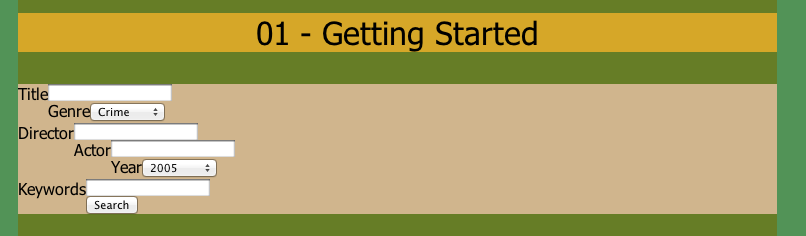
\includegraphics[width=0.9\textwidth]{01-1.png}
\caption{Search interface.}
\label{fig:01-1}
\end{center}
\end{figure}

\begin{figure}[ht]
\begin{center}
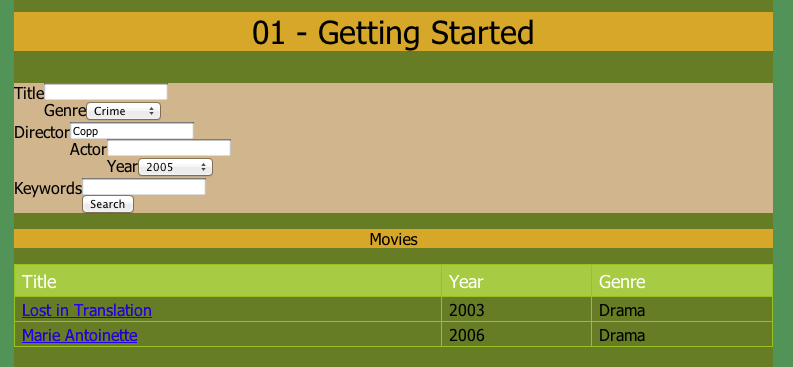
\includegraphics[width=0.9\textwidth]{01-2.png}
\caption{Collapsed search results.}
\label{fig:01-2}
\end{center}
\end{figure}

\begin{figure}[ht]
\begin{center}
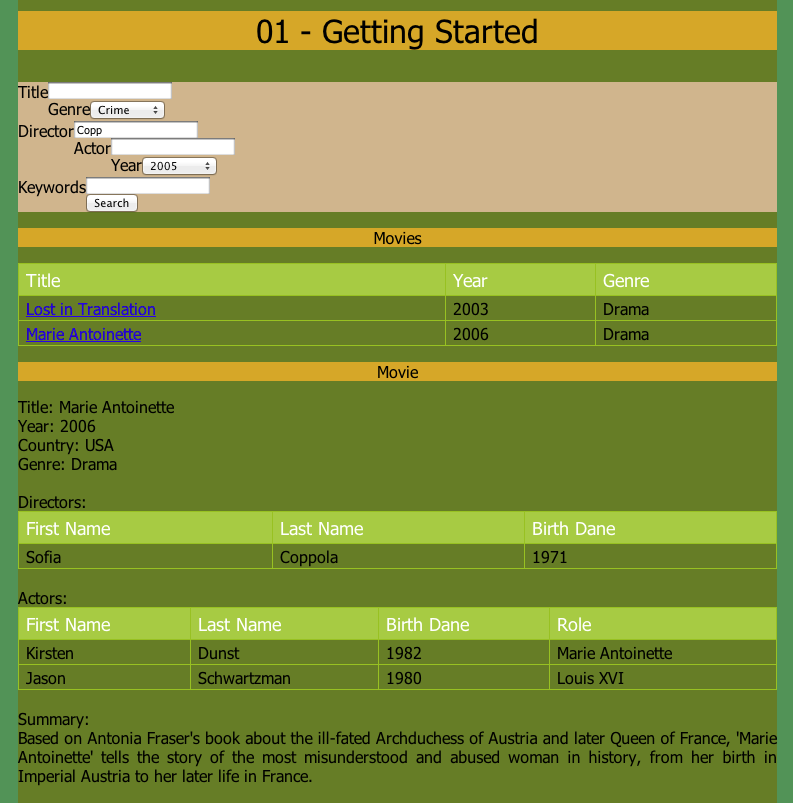
\includegraphics[width=0.9\textwidth]{01-3.png}
\caption{Expanded search results.}
\label{fig:01-3}
\end{center}
\end{figure}

\clearpage
\subsection{Shakespeare Opera Omnia}

The application was built the same way as the first project. You can find the screenshots of a working application at figures 4-8.

The main screen of the application shows the plays that are available for the view. Each play has three associated links, namely Parts, Contents and Summary. Parts interface allows to select a character and view the full text of his role for a given act and scene. Table of Contents view shows all the acts and scenes for a given play in order of their appearance, altogether with the characters participating in a given scene. Summary view shows the author of the play and a full list of participating characters.

\begin{figure}[ht]
\begin{center}

\includegraphics[width=0.9\textwidth]{02-1.png}
\caption{Play selection (main page).}
\label{fig:02-1}
\end{center}
\end{figure}

\begin{figure}[ht]
\begin{center}
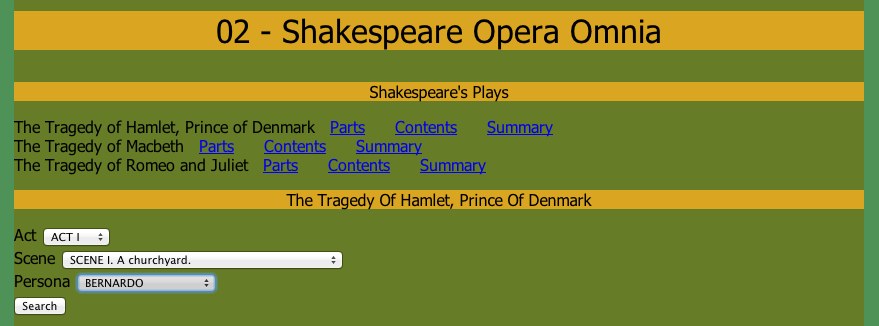
\includegraphics[width=0.9\textwidth]{02-2.png}
\caption{Role selection.}
\label{fig:02-2}
\end{center}
\end{figure}

\begin{figure}[ht]
\begin{center}
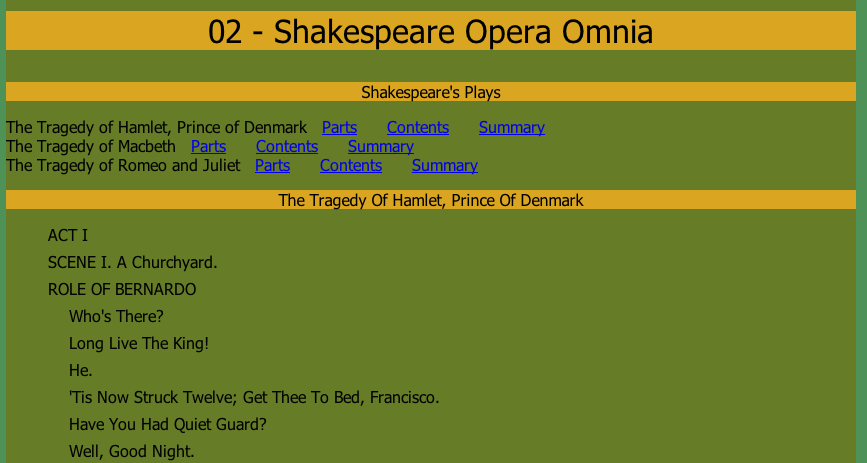
\includegraphics[width=0.9\textwidth]{02-3.png}
\caption{Role view.}
\label{fig:02-3}
\end{center}
\end{figure}

\begin{figure}[ht]
\begin{center}
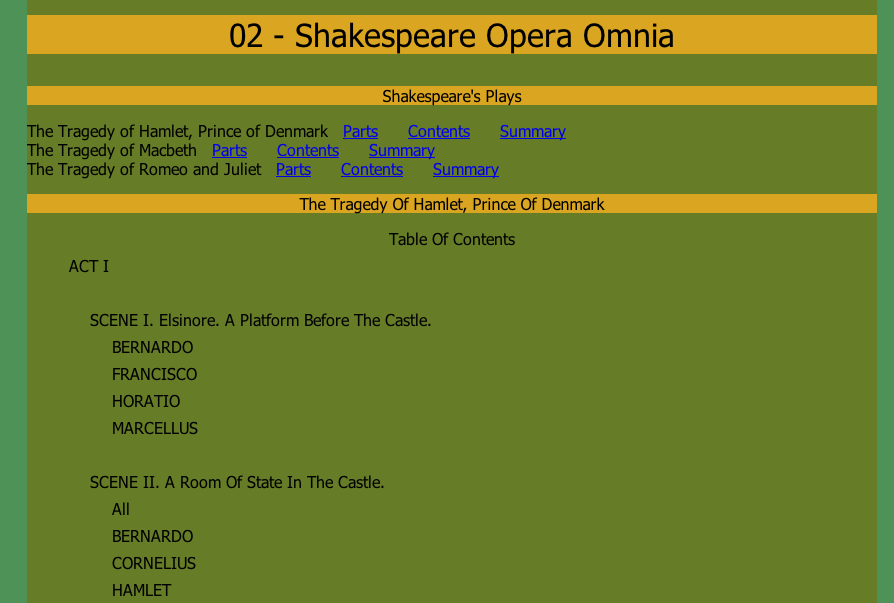
\includegraphics[width=0.9\textwidth]{02-4.png}
\caption{Table of Contents.}
\label{fig:02-4}
\end{center}
\end{figure}

\begin{figure}[ht]
\begin{center}
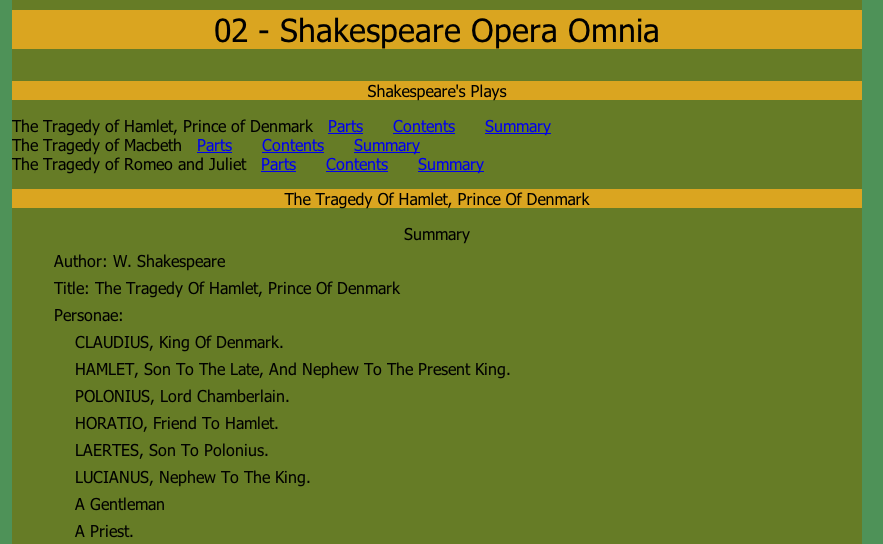
\includegraphics[width=0.9\textwidth]{02-5.png}
\caption{Summary view.}
\label{fig:02-5}
\end{center}
\end{figure}

\clearpage
\subsection{MusicXML on line}

The application was built the same way as the first project. The XML to PDF conversion in done using the ``musicxml2ly'' and ``lilypond'' tools by means of a PHP script, due to JavaScript restrictions. You can find the screenshots of the application at figures 9-10.

The main screen of the application shows the movements that are available to be viewed. Each movement is a link, which when clicked shows more information about the movement, i.e. a short summery, lyrics and the music sheet.

\begin{figure}[ht]
\begin{center}
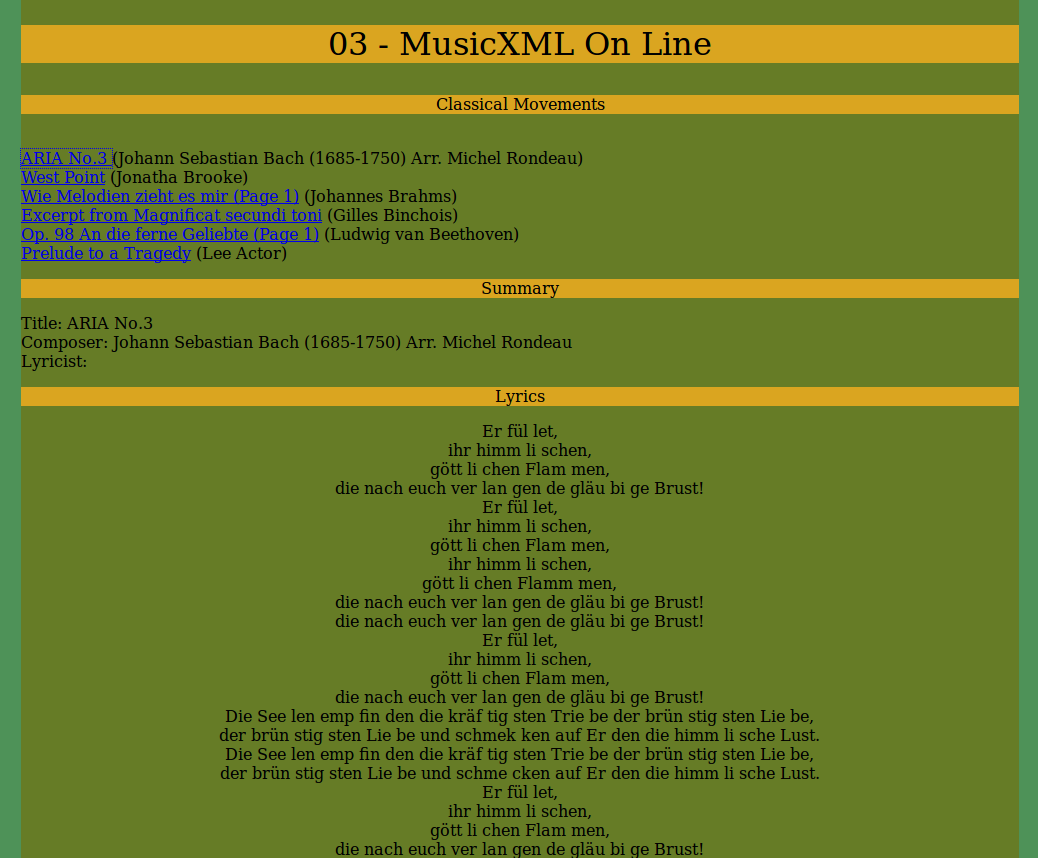
\includegraphics[width=0.9\textwidth]{03-1.png}
\caption{The ``Classical Movements'' section allows you to select a movement for which you would like more information to be displayed.}
\label{fig:03-1}
\end{center}
\end{figure}

\begin{figure}[ht]
\begin{center}
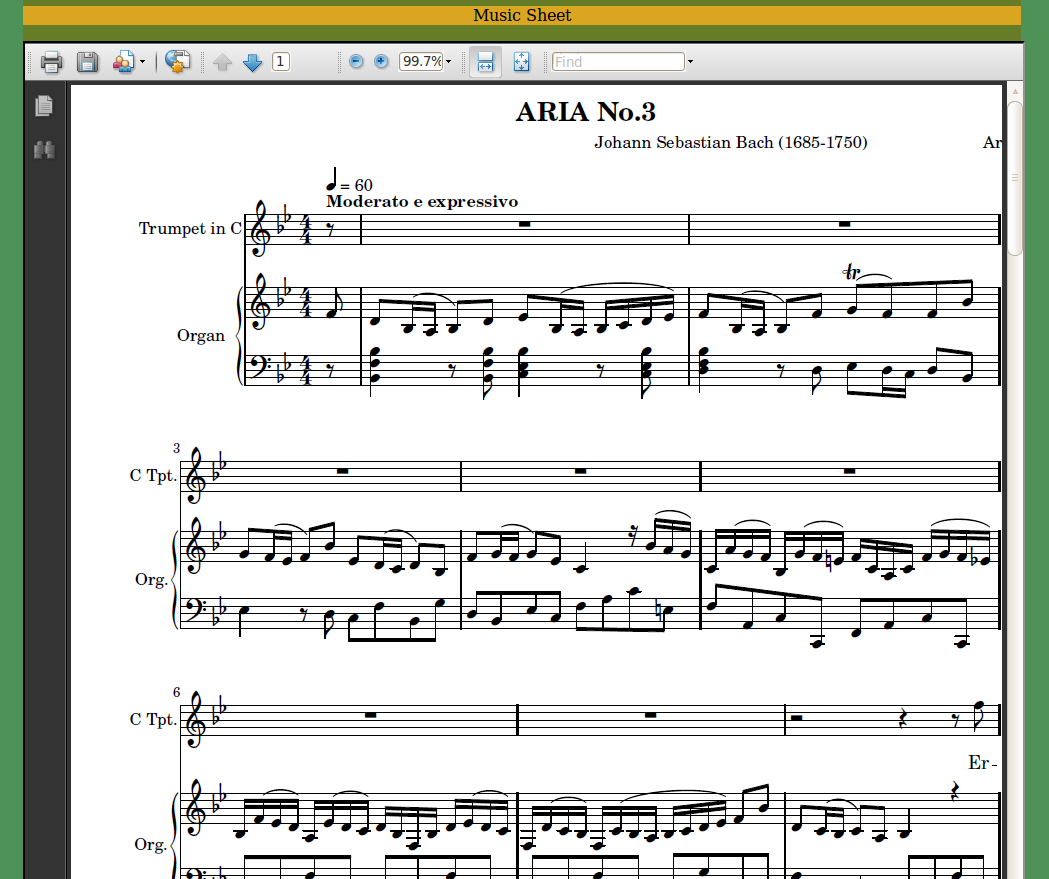
\includegraphics[width=0.9\textwidth]{03-2.png}
\caption{The ``Music Sheet'' section shows the music sheet that is generated using the ``musicxml2ly'' and ``lilypond'' tools by means of a PHP script.}
\label{fig:03-2}
\end{center}
\end{figure}

\end{document}
